%% AISSH-26 manuscript, built on the official sn-jnl.cls template
%% (paper/Archive/sn-jnl.cls, matching the sn-mathphys-num option properly)

\documentclass[pdflatex,sn-mathphys-num]{sn-jnl-official}% official class, numbered Math/Phys reference style

\usepackage{graphicx}%
\usepackage{multirow}%
\usepackage{amsmath,amssymb,amsfonts}%
\usepackage{amsthm}%
\usepackage{mathrsfs}%
\usepackage{xcolor}%
\usepackage{textcomp}%
\usepackage{manyfoot}%
\usepackage{booktabs}%
\usepackage{enumitem}%
\usepackage{float}%

\raggedbottom
\addtolength{\textheight}{25mm}% reclaim unused bottom margin to fit within the page budget
\renewcommand{\arraystretch}{0.72}
\setlist{nosep}

\begin{document}

\title[Safety-Gated, Age-Adaptive LoRA Fine-Tuning for a Virtual Pediatric Hospital Guide]{Safety-Gated, Age-Adaptive LoRA Fine-Tuning for a Virtual Pediatric Hospital Guide}

\author*[1]{\fnm{Anthony} \sur{Barros}}\email{abarros6@uwo.ca}

\author[1]{\fnm{Kelsey} \sur{Kloosterman}}\email{kkloost2@uwo.ca}

\author[2,3]{\fnm{Sandrine} \sur{de Ribaupierre}}\email{sderibau@uwo.ca}

\author[1]{\fnm{Roy} \sur{Eagleson}}\email{eagleson@uwo.ca}

\affil*[1]{\orgdiv{Department of Artificial Intelligence and Software Engineering, Faculty of Engineering}, \orgname{Western University}, \orgaddress{\street{1151 Richmond Street}, \city{London}, \postcode{N6A3K7}, \state{Ontario}, \country{Canada}}}

\affil[2]{\orgdiv{Centre for Brain and Mind}, \orgname{Western University}, \orgaddress{\street{1151 Richmond Street}, \city{London}, \postcode{N6A3K7}, \state{Ontario}, \country{Canada}}}

\affil[3]{\orgdiv{Clinical Neurological Sciences}, \orgname{Western University}, \orgaddress{\street{1151 Richmond Street}, \city{London}, \postcode{N6A3K7}, \state{Ontario}, \country{Canada}}}

\abstract{Pediatric conversational AI requires age-appropriate communication and robust input defense, yet general-purpose safety classifiers fail catastrophically when transferred to pediatric contexts. We present an age-adaptive conversational pipeline comprising the \textit{small-bear conversational model} and the \textit{guard-bear safety layer}, deployed within a digital recreation of Victoria Hospital on an Apple Mac Mini M4 (16~GB) without cloud dependencies. Evaluating the unmodified base classifier \texttt{Prompt-Guard-86M}~\cite{promptguard2024} reveals a failure to transfer to pediatric domain inputs (ROC-AUC 0.448; worse than random due to false-positive saturation). Fine-tuning the \textit{guard-bear classifier} on 4{,}053 pediatric-specific labeled examples restores robust discrimination across a 5-seed campaign (ROC-AUC $0.9992\pm0.0005$, recall $0.988\pm0.004$). For response generation, fine-tuning Llama 3.2 Instruct (1B, 3B) using LoRA (Standard: $r=8$, 16 layers; Fast: $r=4$, 8 layers) on 1,123 synthetic hospital-grounded examples achieves high readability pass rates for ages 5--11 (56--66\% FK~$\leq$~7.0 vs.\ 12\% zero-shot) and distinct inter-role lexical separation (0.92--0.96 vs.\ 0.64--0.67). A prompted baseline achieves comparable readability (92--98\%) and separation (0.970--1.000) but requires 1.2--2.2$\times$ token length, exceeding the 1.0-second latency constraint; adding a strict length clause resolves latency on 1B but reduces inter-role separation (0.870). Fine-tuning eliminates reliance on prompt-engineered length controls while achieving low latency, with the Fast \textit{small-bear model} (1B) meeting the sub-second target on average for ages 5--11. A 110-run multi-seed campaign confirms a configuration-ordering crossover (Fast outperforming Standard on 1B; Standard outperforming Fast on 3B), where the 1B effect reflects a length-independent register shift while the 3B advantage is primarily driven by response length ($p=0.055$ when length-controlled). These findings establish that domain-specific input safety classification is necessary for deployment, and that on-device fine-tuning provides predictable low-latency performance for pediatric applications.}

\keywords{parameter-efficient fine-tuning, low-rank adaptation, pediatric clinical NLP, virtual reality, on-device inference, small language models, LLM input safety classification}

\maketitle

\section{Introduction}\label{sec1}

Deploying large language models (LLMs) in clinical and pediatric environments requires simultaneously managing hardware memory limitations, real-time latency requirements, domain adaptation, and input safety for vulnerable populations. Pediatric conversational systems accepting free-text inputs face unique threat vectors and query distributions that differ substantially from adult and developer-focused LLM applications.

This work introduces an age-adaptive pediatric conversational system composed of two principal artifacts: the \textit{small-bear conversational model}, an age-stratified response generator targeting children (ages 5--11) and adolescents (ages 12--18) in a virtual reality (VR) hospital setting, and the \textit{guard-bear safety layer}, an upstream input classifier. Both components run locally on consumer-grade hardware (Apple Mac Mini M4, 16~GB RAM) to eliminate external cloud dependencies and data transmission risks.

Deploying open-ended text interaction for pediatric populations requires specialized input screening. Standard prompt-injection classifiers, such as \texttt{Prompt-Guard-86M}~\cite{promptguard2024}, focus primarily on system-prompt overrides and developer threat models. Consequently, unadapted base models fail to handle pediatric domain inputs, which consist of short first-person queries, benign out-of-scope questions, and developmental language mixed with out-of-domain content. Fine-tuning the \textit{guard-bear classifier} resolves this transfer failure, establishing robust domain-specific safety gating.

To construct the \textit{small-bear conversational assistant}, Llama 3.2 Instruct models~\cite{dubey2024llama3} (1B and 3B parameter scales) were adapted using Low-Rank Adaptation (LoRA)~\cite{hu2022lora} and QLoRA~\cite{dettmers2023qlora}. Following the LIMA hypothesis~\cite{zhou2023lima}, the model was trained on 1,123 synthetic instruction-response pairs derived from institutional patient resources. We systematically evaluate two adapter parameterizations---Standard ($r=8$, 16 layers) and Fast ($r=4$, 8 layers)---across model scales and age roles.

Experimental evaluation revealed a LoRA configuration-ordering crossover: the Fast configuration achieved superior readability performance on the 1B model, whereas the Standard configuration performed better on the 3B model. A 110-run multi-seed campaign confirmed the empirical validity of this crossover across both model sizes (Section~\ref{sec:seedcampaign}).

\medskip\noindent The main contributions of this paper are:
\begin{itemize}
    \item \textbf{Safety Transfer Analysis and Gating}: We demonstrate that general-purpose safety classifiers fail to transfer to pediatric conversational domains (ROC-AUC 0.448 for the unmodified base model) and show that fine-tuning the \textit{guard-bear classifier} restores high discriminative performance ($0.9992\pm0.0005$ ROC-AUC across 5 seeds).
    \item \textbf{On-Device Age-Adaptive Pipeline}: We implement and evaluate a complete, safety-gated pediatric conversational system running entirely on consumer hardware, comparing fine-tuned adapters against zero-shot and length-constrained prompted baselines to establish trade-offs between latency, readability, and style separation.
    \item \textbf{LoRA Configuration-Ordering Crossover}: We identify and statistically validate a configuration crossover between 1B and 3B parameter models using a 110-run multi-seed campaign, showing that the 1B performance shift represents a length-independent register effect, whereas the 3B shift is predominantly length-driven.
    \item \textbf{Structural Sweeps and Architectural Generalization}: We analyze rank and layer-depth dynamics across sub-7B parameter architectures (Llama 3.2, Qwen 2, SmolLM2, Qwen 2.5), isolating structural depth preferences and evaluating architectural generalization.
\end{itemize}

\section{Related Work}\label{sec:relatedwork}

General-purpose input classifiers such as \texttt{Prompt-Guard-86M}~\cite{promptguard2024} focus on adversarial jailbreak patterns and system-prompt override attempts. Open-source pediatric efforts like \textit{KidRails}~\cite{kidrails2025} apply full fine-tuning to 8B models without separate input classification layers or systematic baseline comparisons. Evaluating dedicated input classifiers against specialized pediatric threat taxonomies remains unaddressed in prior peer-reviewed literature.

Prompted base LLMs have been evaluated for pediatric health communication: Rao et al.~\cite{rao2025pediatric} observed that general models can generate appropriate surgical explanations but highlighted the necessity of domain adaptation, while Hassan et al.~\cite{hassan2025childconv} noted that zero-shot outputs frequently exceed target reading levels. Specialized pretraining approaches such as \textit{KidLM}~\cite{nayeem2024kidlm} adapt masked language models to child-oriented corpora but do not target real-time clinical generation. While virtual reality interventions reduce pediatric procedural anxiety~\cite{ryu2021vr}, existing deployments rely primarily on static scripted content rather than age-adapted, fine-tuned conversational models.

Parameter-efficient fine-tuning via LoRA~\cite{hu2022lora} and QLoRA~\cite{dettmers2023qlora} is widely applied for constrained deployment. However, foundational hyperparameter guidelines---including the comprehensive empirical study by Biderman et al.~\cite{biderman2024lora}---focus on models ranging from 7B to 70B parameters. The interaction between LoRA rank, adapter depth, and capacity regimes in sub-7B models remains under-examined, a gap addressed by our structural sweeps (Section~\ref{sec:ranksweep}).

\section{Results}\label{sec2}

\subsection{small-bear Model Performance: Readability, Latency, and Style Separation}\label{sec:responsemodel}

Table~\ref{tab:res2} reports performance metrics across model configurations on a representative single run (seed 42). Multi-seed statistical validation of the primary crossover effect is detailed in Section~\ref{sec:seedcampaign}. All four fine-tuned configurations outperform zero-shot base models on Flesch-Kincaid (FK) pass rates ($\leq 7.0$) for the 5--11 age group (56--66\% vs.\ 12\%) and demonstrate clear inter-role style separation (Standard-1B/3B: 0.950/0.930; Fast-1B/3B: 0.960/0.920 vs.\ Base-1B/3B: 0.670/0.640).

Prompting the un-adapted base model with an explicit age-targeted system prompt\footnote{Age 5--11: ``You are Dr.\ Beary Good, a warm and friendly guide at a children's hospital. You are talking to a child between the ages of 5 and 11. Use simple words, short sentences, and a warm, reassuring tone.'' Age 12--18: ``You are talking to a teenager between the ages of 12 and 18. Use clear, respectful language appropriate for a teen audience.''} achieves high FK pass rates (92--98\%) and style separation (0.970--1.000). However, unconstrained prompting increases average response length (145--250 tokens vs.\ 87--163 tokens for fine-tuned adapters), elevating inference latency to 2.0--10.3 seconds and reducing sub-second turn rates to 0--8\% (compared to 62\% for the Fast \textit{small-bear model} 1B).

Appending a length-constraint clause (``Keep your answer under 60 words'') to the system prompt reduces 1B latency (0.64s average; 100\% sub-second turns) and maintains readability (100\% FK pass rate), though inter-role style separation declines to 0.870. On the 3B model, adding the length clause reduces latency (1.48s average) but fails to meet the sub-second target (0\% sub-second turns) while achieving 94\% FK pass rate and 0.940 separation.

Fine-tuning eliminates the need for manual, prompt-based length tuning to achieve latency constraints. Among the fine-tuned variants, the Fast \textit{small-bear conversational model} (1B) is the only configuration that achieves an average latency below the 1.0-second interactive VR threshold (0.97s average; 62\% sub-second turns); all 3B configurations average over 2.2 seconds. Evaluated on single-run perplexity, Fast configurations exhibit lower perplexity than Standard across both model scales (1B: 30.18 vs.\ 30.46; 3B: 22.91 vs.\ 24.88).

In single-run evaluation, the Fast \textit{small-bear model} (1B) achieves a higher FK pass rate than the Standard 1B model (62\% vs.\ 56\%), whereas 3B variants perform identically (66\% vs.\ 66\%). The comprehensive multi-seed campaign in Section~\ref{sec:seedcampaign} provides formal statistical bounds for these configuration differences.

\begin{table*}[!h]
  \caption{Readability (50 age-matched held-out prompts/group) and latency/throughput (sequential, Mac Mini M4), single run (seed 42). FK$\leq$7.0 is calibrated to the younger age band (5--11). Prompted-\{1B,3B\} indicates zero-shot base models with age-targeted system prompts without fine-tuning.}
  \label{tab:res2}
  \scriptsize
  \setlength{\tabcolsep}{3pt}
  \begin{tabular}{@{}llcccccccc@{}}
    \toprule
    Config. & Age & FK & SMOG & G.Fog & C-L & TTR & FK$\leq$7.0 & Avg Lat.(s) & $<$1.0s \\
    \midrule
    Standard-1B & 5--11  & 7.1  & 9.2  & 8.7  & 7.1  & 0.756 & 56\% & 1.12 & 26\% \\
    Standard-1B & 12--18 & 10.3 & 12.7 & 13.0 & 10.7 & 0.734 & ---  & 1.36 & 2\%  \\
    Standard-3B & 5--11  & 6.6  & 8.9  & 8.1  & 7.1  & 0.781 & 66\% & 2.22 & 0\%  \\
    Standard-3B & 12--18 & 10.4 & 12.8 & 12.9 & 10.6 & 0.733 & ---  & 3.08 & 0\%  \\
    Fast-1B     & 5--11  & 6.5  & 9.0  & 8.0  & 6.8  & 0.752 & 62\% & 0.97 & 62\% \\
    Fast-1B     & 12--18 & 9.7  & 12.2 & 12.1 & 10.0 & 0.725 & ---  & 1.11 & 38\% \\
    Fast-3B     & 5--11  & 6.5  & 9.0  & 8.1  & 7.1  & 0.724 & 66\% & 2.70 & 0\%  \\
    Fast-3B     & 12--18 & 10.0 & 12.5 & 12.5 & 10.4 & 0.663 & ---  & 3.63 & 0\%  \\
    Base-1B     & 5--11  & 9.5  & 11.9 & 12.0 & 9.6  & 0.582 & 12\% & 1.90 & 16\% \\
    Base-1B     & 12--18 & 10.4 & 12.9 & 13.1 & 11.6 & 0.553 & ---  & 2.23 & 2\%  \\
    Base-3B     & 5--11  & 9.8  & 12.4 & 12.5 & 10.2 & 0.609 & 12\% & 4.54 & 8\%  \\
    Base-3B     & 12--18 & 11.7 & 13.6 & 14.7 & 11.4 & 0.551 & ---  & 5.40 & 2\%  \\
    Prompted-1B & 5--11  & 4.5  & 7.1  & 5.8  & 5.2  & 0.612 & 98\% & 1.97 & 8\%  \\
    Prompted-1B & 12--18 & 7.4  & 10.0 & 9.3  & 7.7  & 0.569 & ---  & 2.22 & 2\%  \\
    Prompted-3B & 5--11  & 4.7  & 7.5  & 6.2  & 5.6  & 0.661 & 92\% & 5.03 & 0\%  \\
    Prompted-3B & 12--18 & 8.4  & 11.3 & 10.6 & 8.8  & 0.581 & ---  & 10.29& 0\%  \\
    \bottomrule
  \end{tabular}
\end{table*}

\subsection{guard-bear Safety Classification Performance}\label{sec:guardresults}

Evaluating the baseline \texttt{Prompt-Guard-86M} model (threshold 0.50) on the 608-example held-out test set demonstrates that general-purpose input safety classifiers fail to transfer to pediatric interaction domains (Table~\ref{tab:guardheadline}). The unmodified base model performs below random chance (ROC-AUC 0.448). This performance occurs because the base model's imperative-override representations do not align with pediatric input characteristics, leading to systematic over-classification of safe inputs as unsafe (flagging 292 of 299 benign samples).

Fine-tuning the \textit{guard-bear classifier} resolves this transfer failure. Across a 5-seed evaluation campaign (Table~\ref{tab:guardheadline}), the fine-tuned model achieves an ROC-AUC of $0.9992\pm0.0005$ and an unsafe recall of $0.9883\pm0.0043$, meeting operational performance targets (recall $\geq 0.97$, precision $\geq 0.85$, F1 $\geq 0.90$, accuracy $\geq 0.92$) across all individual seeds. A TF-IDF with logistic regression baseline trained on identical data achieves 0.9911 ROC-AUC but yields higher total errors (32 vs.\ 6 errors at seed 42; average $\sim$7.8 errors/run across 5 seeds). Fine-tuning demonstrates substantial gains on challenging categories such as \texttt{gibberish\_malformed} inputs (recall increasing from 38\% to 92\%).

Evaluating source provenance across dataset subsets shows high performance on both synthetic unsafe inputs (98.3\% recall) and public unsafe corpora (100\% recall). Optimal classification thresholds vary across training seeds (ranging from 0.04 to 0.94) while maintaining consistent classification performance, establishing that threshold re-calibration is necessary following model retraining.

\begin{table}[!h]
  \centering
  \caption{Performance of the \textit{guard-bear classifier} compared to the base model and TF-IDF+LR baseline on the held-out test set (608 examples: 299 safe, 309 unsafe; deduplicated). The TF-IDF+LR baseline is trained on the same 2{,}836 training subset. The rightmost column reports mean $\pm$ SD across a 5-seed campaign (42, 123, 456, 789, 2024).}
  \label{tab:guardheadline}
  \small
  \begin{tabular}{@{}lcccc@{}}
    \toprule
    Metric & Base (t=0.50) & TF-IDF+LR & Seed 42 & guard-bear (5-seed) \\
    \midrule
    Unsafe recall    & 0.9385 & 0.9644 & 0.9903 & \textbf{0.9883$\pm$0.0043} \\
    Unsafe precision & 0.4983 & 0.9342 & 0.9903 & \textbf{0.9864$\pm$0.0062} \\
    Unsafe F1        & 0.6510 & 0.9490 & 0.9903 & \textbf{0.9874$\pm$0.0049} \\
    Accuracy         & 0.4885 & 0.9474 & 0.9901 & \textbf{0.9872$\pm$0.0050} \\
    ROC-AUC          & 0.4477 & 0.9911 & 0.9998 & \textbf{0.9992$\pm$0.0005} \\
    \bottomrule
  \end{tabular}
  \qquad
  \begin{tabular}{@{}lcccc@{}}
    \toprule
    Confusion & Base & TF-IDF+LR & Seed 42 & 5-Seed Sum ($n$=3040) \\
    \midrule
    TN & 7   & 278 & 296 & 1474 \\
    FP & 292 & 21  & 3   & 21 \\
    FN & 19  & 11  & 3   & 18 \\
    TP & 290 & 298 & 306 & 1527 \\
    \bottomrule
  \end{tabular}
\end{table}

\label{sec:deployment}The combined system footprint operates efficiently on a single local machine. The \textit{guard-bear safety layer} adds minimal processing latency (42.05ms average), enabling the complete pipeline---when paired with the Fast \textit{small-bear conversational assistant} (1B)---to maintain sub-second response times.

\subsection{Statistical Validation of the Configuration-Ordering Crossover}\label{sec:seedcampaign}

To rigorously evaluate the LoRA configuration crossover observed during initial trials, we executed a multi-seed training campaign. Standard ($r=8$, \texttt{num\_layers=16}) and Fast ($r=4$, \texttt{num\_layers=8}) configurations were trained across independent random seeds on the 5--11 age role dataset, measuring FK~$\leq$~7.0 pass rates.

For the 1B \textit{small-bear model}, 25 independent runs per configuration were executed. For the 3B model, an initial batch of 15 seeds per configuration ($t=2.01$, $p=0.054$) was expanded with a planned addition of 15 additional seeds, evaluated using an equal-weight inverse-normal combination test with fixed stage weights.

\begin{table}[!h]
  \centering
  \caption{Multi-seed campaign FK$\leq$7.0 pass rates (mean $\pm$ SD across independent training runs for age 5--11).}
  \label{tab:seedcampaign}
  \small
  \begin{tabular}{@{}lccc@{}}
    \toprule
    Config. & $n$ & Mean & SD \\
    \midrule
    Fast-1B     & 25 & 63.4\% & 6.3 \\
    Standard-1B & 25 & 52.1\% & 6.3 \\
    Fast-3B     & 30 & 52.2\% & 7.0 \\
    Standard-3B & 30 & 58.3\% & 6.9 \\
    \bottomrule
  \end{tabular}
\end{table}

The multi-seed results (Table~\ref{tab:seedcampaign}) confirm the statistical validity of the configuration crossover. On the 1B model, the Fast adapter significantly outperforms the Standard adapter ($t=6.40$, $p=6.0\times10^{-8}$). On the 3B model, the combination test confirms that the Standard adapter outperforms the Fast adapter ($p=0.0015$).

Analyzing all 5{,}500 generated campaign outputs reveals underlying length dynamics. On 1B models, Fast adapters generate shorter responses than Standard adapters (72 vs.\ 78 words average, $p=4\times10^{-16}$), whereas on 3B models, Fast adapters generate longer responses than Standard adapters (97 vs.\ 76 words average, $p=9\times10^{-50}$). Controlling for word count via linear regression demonstrates that the 1B performance gap remains statistically significant after length adjustment (0.35 FK grade level difference, $t=-5.95$, $p=3\times10^{-9}$). Conversely, controlling for response length on the 3B model reduces the configuration gap to 0.10 FK grade levels ($t=-1.92$, $p=0.055$). Logistic regression modeling confirms that the configuration coefficient remains robust at 1B (0.35) but diminishes at 3B (0.007) when word count is included. Thus, the 1B crossover reflects a structural register adaptation, while the 3B difference is primarily mediated by output length.

\subsection{Structural Sweeps: Rank and Layer Depth}\label{sec:ranksweep}

Because Standard and Fast configurations vary both rank ($r$) and targeted layer count (\texttt{num\_layers}), structural sweeps were performed to evaluate their individual contributions. Sweeps were conducted across two independent seeds per configuration using the updated dataset vintage.

Fixing \texttt{num\_layers=8} while sweeping rank $r \in \{2,4,8,16\}$ across four architectures (Table~\ref{tab:sweeps}, left) reveals model-specific variations. SmolLM2 360M exhibits monotonic performance improvements with increasing rank (48\% to 63\% pass rate). In contrast, Llama 3.2 (1B and 3B) and Qwen 2 (0.5B) demonstrate flat or non-monotonic readability responses across rank variations at fixed layer depth.

Sweeping layer depth at fixed rank ($r=4$, \texttt{num\_layers} $\in \{4,8,16\}$; Table~\ref{tab:sweeps}, right) demonstrates distinct depth preferences: 3B models achieve optimal readability at maximum depth (63\% pass rate at 16 layers), whereas 1B models perform best at shallow depth allocations (69\% pass rate at 4 layers, decreasing to 60\% at 16 layers). Across both model sizes, inference latency scales proportionally with targeted layer depth.

\begin{table}[!h]
  \centering
  \caption{Rank sweep (left; fixed \texttt{num\_layers=8}) and layer depth sweep (right; fixed $r=4$) FK $\leq 7.0$ pass rates, reported as mean $\pm$ range across two independent seeds.}
  \label{tab:sweeps}
  \scriptsize
  \setlength{\tabcolsep}{3pt}
  \begin{tabular}{@{}lcccc@{}}
    \toprule
    Model     & $r{=}2$ & $r{=}4$ & $r{=}8$ & $r{=}16$ \\
    \midrule
    Llama 1B  & 63$\pm$10 & 59$\pm$7 & \textbf{64$\pm$6} & 62$\pm$6 \\
    Llama 3B  & 54$\pm$11 & 58$\pm$3 & 57$\pm$1 & \textbf{62$\pm$11} \\
    Qwen 0.5B & 70$\pm$3 & \textbf{71$\pm$13} & 71$\pm$4 & 60$\pm$11 \\
    SmolLM2   & 48$\pm$3 & 56$\pm$6 & 62$\pm$6 & \textbf{63$\pm$4} \\
    \bottomrule
  \end{tabular}
  \qquad
  \begin{tabular}{@{}lccc@{}}
    \toprule
    Model, Layers & FK$\leq$7 & Lat.(s) & Tok/s \\
    \midrule
    1B, 4  & \textbf{69\%} & 0.85 & \textbf{105.6} \\
    1B, 8  & 61\% & 0.84 & 97.4 \\
    1B, 16 & 60\% & 1.06 & 84.0 \\
    3B, 4  & 57\% & 2.73 & \textbf{45.0} \\
    3B, 8  & 60\% & 2.67 & 43.2 \\
    3B, 16 & \textbf{63\%} & \textbf{2.24} & 39.5 \\
    \bottomrule
  \end{tabular}
\end{table}

\subsection{Cross-Architecture Evaluation}\label{sec:crossarch}

Cross-architecture generalization was evaluated using Qwen 2 (0.5B), SmolLM2 (360M), and the Qwen 2.5 model family (0.5B, 1.5B, 3B) on the age 5--11 task (Table~\ref{tab:crossarch}). SmolLM2 Standard achieves an 80\% FK pass rate. Across the Qwen 2.5 family, Fast configurations match or exceed Standard configurations at every model scale (e.g., 74\% vs.\ 66\% at 1.5B; 70\% vs.\ 50\% at 3B), indicating that the configuration crossover observed in Llama 3.2 does not extend to the Qwen 2.5 architecture family.

\begin{table*}[!h]
  \centering
  \caption{Cross-architecture performance for age 5--11 (50 examples, seed 42). Style-Sep.\ measures inter-role lexical separation via 5-fold cross-validation ($\dagger$indicates original pre-revision dataset baseline).}
  \label{tab:crossarch}
  \scriptsize
  \setlength{\tabcolsep}{3pt}
  \begin{tabular}{@{}lccccc@{}}
    \toprule
    Config. & FK$\leq$7.0 & Avg Lat. & $<$1.0s & Tok/s or Tok & Style-Sep.$^\dagger$ \\
    \midrule
    Qwen 2 Std.       & 68\% & 0.54\,s & 100\% & 83 tok  & $0.940 \pm 0.049$ \\
    Qwen 2 Fast       & 62\% & 0.51\,s & 96\%  & 94 tok  & $0.960 \pm 0.058$ \\
    SmolLM2 Std.      & 80\% & 0.87\,s & 72\%  & 82 tok  & $0.950 \pm 0.032$ \\
    SmolLM2 Fast      & 60\% & 1.30\,s & 56\%  & 137 tok & $0.920 \pm 0.040$ \\
    Qwen2.5-0.5B Fast & 56\% & 0.45\,s & 100\% & 176.4   & $0.950 \pm 0.032$ \\
    Qwen2.5-0.5B Std. & 56\% & 0.57\,s & 100\% & 152.1   & $0.940 \pm 0.097$ \\
    Qwen2.5-1.5B Fast & 74\% & 1.07\,s & 58\%  & 76.1    & $\mathbf{0.980 \pm 0.024}$ \\
    Qwen2.5-1.5B Std. & 66\% & 1.28\,s & 6\%   & 67.8    & $0.890 \pm 0.073$ \\
    Qwen2.5-3B Fast   & 70\% & 1.73\,s & 4\%   & 43.0    & $0.970 \pm 0.040$ \\
    Qwen2.5-3B Std.   & 50\% & 2.18\,s & 0\%   & 39.9    & $0.930 \pm 0.068$ \\
    \bottomrule
  \end{tabular}
\end{table*}

\section{Methods}\label{sec:methodology}

\subsection{System Architecture}\label{sec:architecture}

The system pipeline processes input through two sequential stages (Figure~\ref{fig:architecture}). Raw text is first evaluated by the \textit{guard-bear safety layer}. Inputs classified as unsafe are intercepted and returned with standard safety handling. Safe inputs pass through an age router provided by the host VR application, which selects the corresponding fine-tuned adapter on a frozen 4-bit quantized base model. System prompts are omitted during adapter inference to ensure that age-specific register is encoded directly within adapter weights.

\setlength{\intextsep}{2pt}
\setlength{\textfloatsep}{4pt}
\setlength{\abovecaptionskip}{2pt}
\setlength{\belowcaptionskip}{0pt}
\begin{figure}[H]
  \centering
  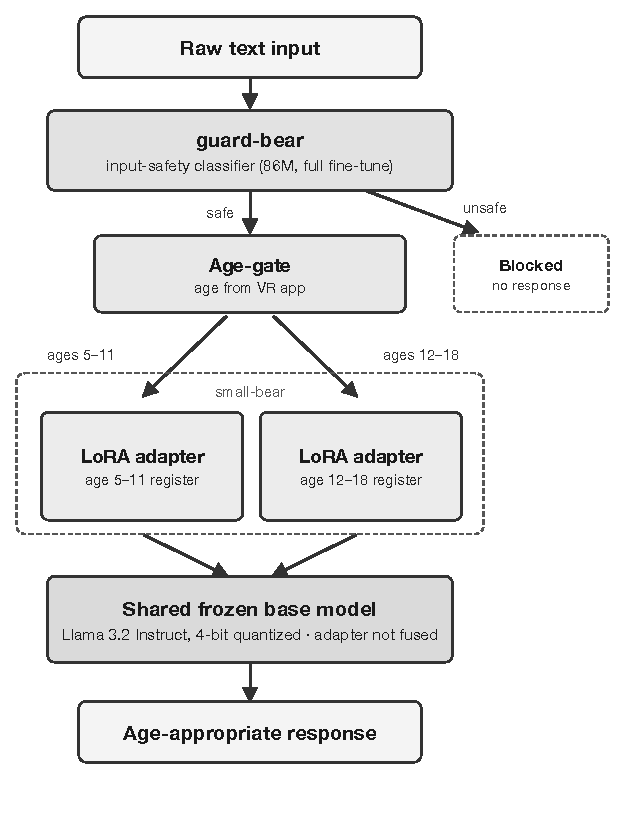
\includegraphics[width=0.36\textwidth]{images/architecture_adapters_router.pdf}
  \caption{System architecture diagram. The \textit{guard-bear safety layer} (86M parameters) screens incoming text before routing safe queries to age-stratified LoRA adapters deployed on a frozen 4-bit Llama 3.2 base model.}
  \label{fig:architecture}
\end{figure}

The \textit{guard-bear classifier} performs full parameter fine-tuning of an 86M parameter DeBERTa architecture to categorize inputs as safe (benign pediatric questions and out-of-scope curiosity) or unsafe (adversarial injections, adult themes, and malformed text). Single-query evaluation averages 42.05ms on the target hardware platform.

\subsection{Datasets}\label{subsec:responsedataset}

Training data for the \textit{small-bear conversational assistant} was constructed from institutional patient education materials~\cite{hospitalguide}. The dataset comprises 1,123 instruction-response pairs split across two age targets (562 for ages 5--11; 561 for ages 12--18), supplemented by 100 validation examples and 50 training-only edge-case entries.

The \textit{guard-bear classifier} training set combines synthetic pediatric queries with established safety corpora, yielding 4{,}053 unique, deduplicated samples (2{,}055 unsafe, 1{,}998 safe) partitioned into disjoint train (2,836), validation (609), and test (608) splits.

\subsection{Base Models, LoRA Configurations, and Training Protocol}\label{sec:trainprotocol}

Fine-tuning of the \textit{small-bear conversational model} was conducted using 4-bit quantized Llama 3.2 Instruct base models (1B and 3B) via \texttt{mlx\_lm}~\cite{apple2023mlx}. LoRA updates ($\Delta W = BA$) were applied to linear projections across target layers with scaling factor fixed at \texttt{scale=20.0}. The **Standard** configuration parameterizes $r=8$ across the upper 16 layers, while the **Fast** configuration parameterizes $r=4$ across the upper 8 layers. Optimization used Adam with cosine learning rate decay (peak $1\times10^{-5}$, 100-step warmup, 600 total steps, batch size 4).

The \textit{guard-bear safety layer} was fine-tuned from \texttt{Prompt-Guard-86M}~\cite{promptguard2024}. The classification decision threshold was optimized on validation performance, establishing an operational threshold of **0.94**.

\subsection{Evaluation Methodology}

Readability metrics for the \textit{small-bear model} were evaluated using \texttt{textstat}~\cite{bansal2023textstat}, establishing Flesch-Kincaid (FK~$\leq$~7.0) as the primary benchmark alongside SMOG, Gunning Fog, Coleman-Liau, and Type-Token Ratio (TTR). Inter-role lexical separation was evaluated via 5-fold cross-validated TF-IDF logistic regression classifiers. The \textit{guard-bear classifier} was evaluated on unsafe recall, precision, F1 score, accuracy, ROC-AUC, and subcategory recall.

\section{Discussion}\label{sec:discussion}

The failure of un-adapted safety classifiers on pediatric inputs underscores that **safety mechanisms cannot be assumed to transfer across domain populations without explicit fine-tuning**. The base classifier's low ROC-AUC (0.448) demonstrates that developer-focused threat representations misclassify benign pediatric interactions. Fine-tuning the \textit{guard-bear safety layer} eliminates these false positives while maintaining high unsafe recall ($0.9883\pm0.0043$).

For response generation, the Fast \textit{small-bear conversational assistant} (1B) achieves the operational requirements of interactive VR deployment, sustaining an average latency of 0.97 seconds and a 62\% sub-second turn rate. While length-constrained system prompts enable base models to achieve comparable readability, fine-tuning provides predictable low-latency output without manual prompt engineering.

Statistical analysis of the LoRA configuration crossover confirms distinct architectural behaviors between model scales. The performance advantage of Fast adapters on 1B models reflects a genuine register shift that remains significant after controlling for response length. Conversely, the advantage of Standard adapters on 3B models is primarily mediated by output length reduction.

\section{Conclusion}\label{sec:conclusion}

This study demonstrates that deploying pediatric conversational AI requires domain-specific safety adaptation and tailored model configurations. Unmodified safety classifiers fail to transfer to pediatric input distributions, a limitation resolved by fine-tuning the \textit{guard-bear classifier} to achieve $0.9992\pm0.0005$ ROC-AUC. For response generation, fine-tuning the \textit{small-bear conversational model} yields age-appropriate communication while satisfying on-device sub-second latency constraints. Validating adapter parameterizations across model scales reveals a LoRA configuration crossover, establishing that fine-tuning dynamics in sub-7B models depend on scale-specific interactions between layer depth, rank, and response length.

\textbf{Limitations.} Evaluation is based on automated readability and lexical metrics; clinical efficacy and expert pediatric communication quality remain to be evaluated by human raters. Factual accuracy of generated responses was not formally benchmarked against institutional knowledge bases. End-to-end system latency reflects sequential component evaluations rather than simultaneous pipeline operation. Finally, optimal decision thresholds for the safety layer varied across retraining seeds, necessitating post-hoc threshold calibration whenever the classifier is retrained.

\backmatter

\bmhead{Supplementary Information}

Validation outputs, dataset files, and training scripts are available in the public repositories listed under Data Availability.

\bmhead{Acknowledgements}

Not applicable.

\section*{Declarations}

\begin{itemize}
\item \textbf{Funding:} No external funding was received for this work.
\item \textbf{Conflict of Interest:} The authors declare no competing interests.
\item \textbf{Ethics Approval:} Not applicable. The study utilized synthetic and public datasets without human subjects or clinical interventions.
\item \textbf{Data and Code Availability:} Code and data for the \textit{small-bear conversational model} are available at \url{https://github.com/abarros6/small-bear}. Code and data for the \textit{guard-bear classifier} are available at \url{https://github.com/abarros6/guard-bear}.
\item \textbf{Author Contributions:} S.d.R. and R.E. supervised the research. A.B. designed the experiments, implemented the models, and prepared the manuscript text. K.K. contributed to the introduction and domain framing. All authors reviewed and approved the manuscript.
\end{itemize}

\bibliography{aissh_final}

\end{document}
